%------------------------------------------------------------------------------
%	CAPITOLO 14
%------------------------------------------------------------------------------

\chapter{Da 15 a 20 paoli di stipendio}
La sede del comune era nel \index[Luoghi]{Borghetto}Borghetto (\index[Luoghi]{Lanconelli (palazzo)}casa Lanconelli ora Martini\footnote{In via Mazzini, nel cosiddetto \textbf{Borghetto}, vi è un lungo caseggiato che viene detto  la ‘Ca d'Pliché'. Pliché era il soprannome dei Martini che vi abitarono e che ne sono ancora i proprietari (2017). Essi erano succeduti alla fine dell'ottocento ai proprietari storici di quell'edificio: i Lanconelli.}). Il consiglio comunale si era radunato in seduta segreta per varie trattazioni e per aumentare lo stipendio al bidello\footnote{Qui inteso come custode.} \index[Personaggiq]{Panciaco (bidello)}Panciaco da 15 a 20 paoli al mese. (\Large \textcal{L 7,50 a 10}\normalfont \normalsize \:)\\
\indent Panciaco per chi non lo sapesse era un omone grande e grosso, molto decorativo, vestito alla Napoleone, con lucerna in testa, falde e spada, per le funzioni della messa cantata della domenica, insieme alla magistratura al completo, con guardie e carabinieri, e per le altre funzioni civili, non escluse le sedute consigliari, che serviva nell'anticamera anche con funzioni di guardiaportone.\\
\indent Al termine della seduta, certo dell'aumento al povero Panciaco, tirava anche l'ombellico dalla consolazione dell'agognato aumento.\\
\indent Con la maestà della divisa e di un Napoleone, spalancò la porta dell'aula consigliare e proruppe con questa esclamazione: <<Ringrazio questa nobile plebaglia!>>\\
\indent Si arguisce che il discorso studiato non lo seppe dire o si confuse.

 \begin{figure}[htb]
    \centering
    %\vspace{-0.7cm}
    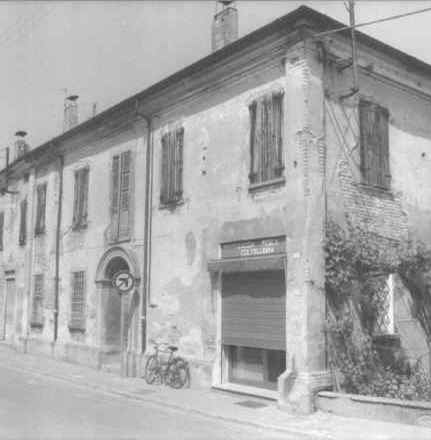
\includegraphics[width=\textwidth]{casamartini}
    \caption[Caseggiato Martini - Lanconelli]{Il \textbf{caseggiato Martini - Lanconelli}. Lanconelli fu una delle più ricche famiglie che fu nel territorio alfonsinese fin dai primi dell’ottocento. Prima di questa data non si hanno notizie della presenza di tale famiglia ad Alfonsine. Probabilmente erano lughesi e, con l’avvento di Napoleone e l’occupazione francese dei territori anche nella Bassa Romagna, riuscirono ad approfittarne. \label{fig:casamartini}}
    %\vspace{-0.3cm}
\end{figure}